\documentclass[a4paper,11pt,dvipdfmx]{ujarticle}
% パッケージ
\usepackage{graphicx}
\usepackage{url}
% レイアウト指定を記述したファイルの読み込み
\input{layout}

% タイトルと氏名を変更せよ.
\title{日本におけるデジタル化の状況}
\author{G584392025 小竹 希}

\begin{document}

\maketitle %ここにタイトルが入る

\section{ブロードバンドの整備状況}

OECDによるブロードバンド回線の普及に関する調査\cite{OECD}によると,
図\ref{fig:加入数}に示すように,
日本における100人あたりのモバイルブロードバンドの加入者数は190.5で、
第1位になっている。2位はエストニアで、3位は米国と続く。

\begin{figure}[htbp]
    \centering
    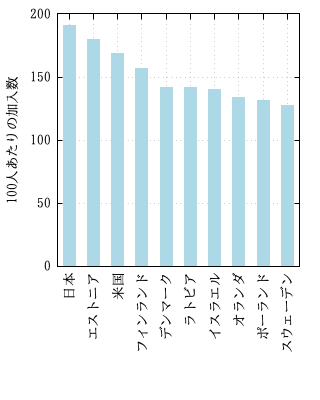
\includegraphics[width=0.6\linewidth]{fig21.png}
    \caption{光ファイバー回線の加入者数}\label{fig:加入数}
\end{figure}

\section{デジタル競争ランキング}

国際経営開発研究所(IMD)の調査\cite{IMD}によると、
日本のデジタル競争力のランキングは
表\ref{tbl:デジタル競争}に示すように,
調査の対象の64カ国中、
総合で28位、技術分野で30位となっている。


\begin{table}[htbp]
    \centering
    \caption{デジタル競争力ランキング(64カ国中)}
    \label{tbl:デジタル競争}

    \begin{tabular}{|c|c|c|}
        \hline
        国 & 総合 & 技術\\
        \hline
        米国 & 1位 & 4位\\
        \hline
        香港 & 2位 & 10位\\
        \hline
        スウェーデン & 3位 & 8位\\
        \hline
        デンマーク & 4位 & 2位\\
        \hline
        シンガポール & 5位 & 3位\\
        \hline
        \hline
        韓国 & 12位 & 13位\\
        \hline
        中国 & 15位 & 20位\\
        \hline
        \hline
        日本 & 28位 & 30位\\
        \hline
    \end{tabular}
\end{table}

\section{考察:IMD 2021年ランキングから読み解く現状}

\begin{itemize}
    \item 全分野で課題は「技術」(30位)、「将来への準備」(29位)も低く、分野横断的な遅れ。
    \item 米国は「将来への準備」で1位、シンガポールは「技術」「将来への準備」で高評価。
    \item アジア競合国との差: 韓国(12位)、中国(15位)が日本(28位)を大きく上回り、アジア内での遅れが顕著。
\end{itemize}

\begin{table}[htbp]
    \centering
    \caption{デジタル競争力ランキング(64カ国中)}

    \begin{tabular}{|c|c|c|c|}
        \hline
        国 & 総合 & 技術 & 将来への準備 \\
        \hline
        米国 & 1位 & 4位 & 1位 \\
        \hline
        香港 & 2位 & 10位 & 2位 \\
        \hline
        スウェーデン & 3位 & 8位 & 3位\\
        \hline
        デンマーク & 4位 & 2位 & 5位 \\
        \hline
        シンガポール & 5位 & 3位 & 4位\\
        \hline
        韓国 & 12位 & 13位 & 11位 \\
        \hline
        中国 & 15位 & 20位 & 18位 \\
        \hline
        日本 & 28位 & 30位 & 29位 \\
        \hline
    \end{tabular}
\end{table}
\bibliographystyle{junsrt}
\bibliography{exercise.bib}

\end{document}